\documentclass[prb,preprint]{revtex4-2} 
% The line above defines the type of LaTeX document.
% Note that AJP uses the same style as Phys. Rev. B (prb).

% The % character begins a comment, which continues to the end of the line.

\usepackage{amsmath}  % needed for \tfrac, \bmatrix, etc.
\usepackage{amsfonts} % needed for bold Greek, Fraktur, and blackboard bold
\usepackage{graphicx} % needed for figures

\begin{document}

% Be sure to use the \title, \author, \affiliation, and \abstract macros
% to format your title page.  Don't use lower-level macros to  manually
% adjust the fonts and centering.

\title{Preparation of manuscripts for the American Journal of Physics
using \LaTeX}
% In a long title you can use \\ to force a line break at a certain location.

%When submitting the manuscript for review, do not include the author's name or institution
%\author{Daniel V. Schroeder}
%\email{dschroeder@weber.edu} % optional
%\altaffiliation[permanent address: ]{101 Main Street, Anytown, USA} % optional second address
% If there were a second author at the same address, we would put another 
% \author{} statement here.  Don't combine multiple authors in a single
% \author statement.
%\affiliation{Department of Physics, Weber State University, Ogden, UT 84408-2508}
% Please provide a full mailing address here.

%\author{David P. Jackson}
%\email{ajp@dickinson.edu}
%\affiliation{Department of Physics, Dickinson College, Carlisle, PA 17013}

% See the REVTeX documentation for more examples of author and affiliation lists.

\date{\today}

\begin{abstract}
This article explains and illustrates the use of \LaTeX\ in preparing manuscripts
for submission to the American Journal of Physics (AJP). While it is not a
comprehensive reference, we hope it will suffice for the needs of most
AJP authors.  For help on a specific question, an internet search engine will 
generally return many useful answers if the term ``latex'' is included in the 
search box.
\end{abstract}
% AJP requires an abstract for all regular article submissions.
% Abstracts are optional for submissions to the "Notes and Discussions" section.

\maketitle % title page is now complete


\section{Introduction} % Section titles are automatically converted to all-caps.
% Section numbering is automatic.

\LaTeX\ is typesetting software that is widely used by mathematicians
and physicists because it is so good at typesetting equations. It is 
also completely programmable, so it can be configured to produce 
documents with almost any desired formatting, and to automatically
number equations, figures, endnotes, and so on.

To prepare manuscripts for the American Journal of Physics (AJP), 
you should use the REV\TeX\ 4.1 format for Physical Review B
preprints, as indicated in the \texttt{documentclass} line at the top 
of this article's source file.  (If you're already familiar with 
\LaTeX\ and have used other \LaTeX\ formats, please resist the 
temptation to use them, or to otherwise override REV\TeX's formatting 
conventions, in manuscripts that you prepare for AJP.)

This sample article is intended as a tutorial, template, and reference for 
AJP authors, illustrating most of the \LaTeX\ and REV\TeX\ features that 
authors will need.  For a more comprehensive introduction to \LaTeX, 
numerous books and online references are available.\cite{latexsite, 
wikibook, latexbook}  Documentation for the REV\TeX\ package 
can be found on the APS web site.\cite{revtex}

\LaTeX\ is free software, available for Unix/Linux, Mac OS X, and Windows
operating systems. For downloading and installation instructions, follow
the links from the \LaTeX\ web site.\cite{latexsite} It is most
convenient\cite{cloudLaTeX} to install a ``complete \TeX\ distribution,'' 
which will include \LaTeX, the underlying \TeX\ engine, macro packages 
such as REV\TeX, a large collection of fonts, and GUI tools for editing 
and viewing your documents.  To test your installation, try to process
this sample article.


\section{Ordinary text and paragraphs}

To typeset a paragraph of ordinary text, just type the text in your source
file like this. Put line breaks
wherever
you
want, and don't      worry      about      extra      spaces      between      words, which \LaTeX\ will ignore.  You can almost always trust \LaTeX\ to make your paragraphs look good, with neatly justified margins.  % Long lines of text are fine, since most editing programs will wrap them automatically.

To start a new paragraph, just leave a blank line in your source file.

A few punctuation characters require special treatment in \LaTeX. There 
are no ``smart quotes,'' so you need to use the left-quote key (at the 
top-left corner of the keyboard) for a left quote, and the ordinary apostrophe
key (next to the semi-colon) for a right quote. Hit either key twice for double
quotes, which are standard in American English.  Don't use shift-apostrophe
to make double quotes.  Use single quotes when they're nested inside a 
double-quoted quotation.  When a period or comma belongs at the end of
a quotation, put it inside the quotes---even if it's not part of what you're
quoting.\cite{nevermindlogic}

Your fingers also need to distinguish between a hyphen (used for
multi-word adjectives and for hyphenated names like Lennard-Jones), an 
en-dash (formed by typing two consecutive hyphens, and used for ranges 
of numbers like 1--100), and an em-dash (formed out of three consecutive
hyphens and used as an attention-getting punctuation symbol---preferably 
not too often).

Some non-alphanumeric symbols like \$, \&, and \% have special meanings 
in a \LaTeX\ source file, so if you want these symbols to appear in the output, 
you need to precede them with a backslash.

There are also special codes for generating the various accents
that can appear in foreign-language words and names, such as Amp\`ere
and Schr\"odinger.\cite{FontEncodingComment}

You can switch to \textit{italic}, \textbf{bold}, and \texttt{typewriter} fonts
when necessary. Use curly braces to enclose the text that is to appear in 
the special font. In general, \LaTeX\ uses curly braces to group characters 
together for some common transformation.

Notice that any word or symbol preceded by the backslash character is
a special instruction to \LaTeX, typically used to produce a special 
symbol or to modify the typeset output in some way. These instructions 
are also called \textit{control sequences} or \textit{macros}.  
After you've used \LaTeX\ for a while, the little finger of your right 
hand will be really good at finding the backslash and curly-brace keys.


\section{Math symbols}

To type mathematical symbols and expressions within a paragraph, put
them between \$ signs, which indicate \textit{math mode}: $ab + 2c/d = e-3f$.
\LaTeX\ ignores spaces in math mode, using its own algorithms to determine
the right amount of space between symbols.  Notice that an ordinary letter 
like~$x$, when used in math mode, is automatically typeset in italics. 
This is why you need to use math mode for all mathematical
expressions (except plain numerals), even when they don't contain any 
special symbols.  But don't use math mode to italicize ordinary \textit{words}.

Besides ordinary letters and numerals and common arithmetic symbols, math 
mode provides a host of other characters that you can access via control 
sequences.\cite{wikimathpage} These include Greek letters like $\pi$ and 
$\Delta$ (note capitalization), symbols for operations and relations such 
as $\cdot$, $\times$, $\pm$, $\gg$, $\leq$, $\sim$, $\approx$, $\propto$, 
and $\rightarrow$, and special symbols like $\nabla$, $\partial$, $\infty$, 
and~$\hbar$. You can decorate symbols with dots ($\dot x$ or $\ddot x$), 
arrows ($\vec\mu$), bars ($\bar x$ or $\overline m$), hats ($\hat x$), 
tildes ($\tilde f$ or $\widetilde w$), and radicals ($\sqrt\pi$, $\sqrt{2/3}$).
Parentheses and square brackets require no special keystrokes, but you
can also make curly braces and angle brackets: $\{\langle\ \cdots\ \rangle\}$.

To make subscripts and superscripts, use the underscore and caret 
(circumflex) symbols on your keyboard: $x^\mu$, $g_{\mu\nu}$, $\delta^i_j$, 
$\epsilon^{ijk}$.  Notice that you need to put the subscript or superscript 
in curly braces if it's longer than one character (or one control sequence). 
You can even make nested subscripts and superscripts, as in $e^{-x^2}$.  
If a subscript consists of an entire word or word-like abbreviation, 
we usually put it in plain Roman type: $x_\textrm{max}$.  If you need to 
put a subscript or superscript \textit{before} a symbol, use an empty
set of curly braces: ${}^{235}_{\ 92}\textrm{U}$. (Notice the trick of using 
backslash-space put a space before the 92.)

\newcommand{\bE}{\mathbf{E}}   % defines the abbreviation \bE, used below

To make boldface letters you use the \verb/\mathbf/ control sequence, as in
$\nabla\times\mathbf{E} = -\partial\mathbf{B}/\partial t$.  For bold Greek
letters like $\boldsymbol{\omega}$, you need to use \verb/\boldsymbol/
instead.  You can also use calligraphic ($\mathcal{E}$), Fraktur 
($\mathfrak{D}$), and blackboard bold ($\mathbb{R}$) fonts, if you need them. 
If you'll be using a symbol in a special font repeatedly, you can save 
some keystrokes by defining an abbreviation for it; for example, the 
definition \verb/\newcommand{\bE}{\mathbf{E}}/ allows you to type simply 
\verb/\bE/ to get $\bE$.

Unit abbreviations, as in $1~\mathrm{eV} = 1.6\times10^{-19}~\mathrm{J}$,
should be in the plain Roman font, not italics.  You can access this font
from math mode using \verb/\mathrm/. For function names like $\sin\theta$, 
$\exp x$, and $\ln N!$, \LaTeX\ provides special control sequences, 
which you should use instead of \verb/\mathrm/ whenever possible because
they work better with \LaTeX's automatic spacing algorithms.

But \LaTeX\ doesn't always get the spacing right in mathematical formulas.
In the previous paragraph we had to use the \verb/~/ symbol to 
manually insert a space between each number and its units.  The \verb/~/
symbol actually represents an unbreakable space, where \LaTeX\ will never
insert a line break. For occasional minor adjustments to the spacing
in a \LaTeX\ expression, you can insert or remove a little 
space with \verb/\,/ and \verb/\!/.  Use these macros sparingly,
because \LaTeX's default spacing rules will provide more consistency
within and among AJP articles.  The most common use of \verb/\,/ 
is in expressions like $T\,dS - P\,dV$.


\section{Displayed equations}
\label{DispEqSection}	% You can label sections for reference

When an equation is important and/or tall and/or complicated, you should 
display it on a line by itself, with a number. To do this, you put 
\verb/\begin{equation}/ before the equation and \verb/\end{equation}/ 
after it, as in     % Note: never put a blank line before an equation.
\begin{equation}
\int_0^\infty \! \frac{x^3}{e^x - 1} \, dx = 6\sum_{k=1}^\infty \frac1{k^4} = 
    6\left(\frac{\pi^4}{90}\right) = \frac{\pi^4}{15}.
\end{equation}
% Don't put a blank line after the equation unless you're starting a new paragraph.
This example also shows how to make the sum and integral symbols, big parentheses, 
% Don't use \left and \right for small parentheses; you'll get too much space around them.
and built-up fractions.  (Don't put built-up fractions in a 
non-displayed equation, because there won't be enough vertical space in 
AJP's final, single-spaced paragraphs.  Use the slashed form, $x^3/(e^x-1)$, 
instead.)

If you want to refer to an equation elsewhere in your manuscript, you can 
give it a label.  For example, in the equation
\begin{equation}
\label{deriv}
\frac{\Delta x}{\Delta t} \mathop{\longrightarrow}_{\Delta t\rightarrow0} \frac{dx}{dt} 
 = \lim_{\Delta t\rightarrow0} \frac{\Delta x}{\Delta t}
\end{equation}
we've inserted \verb/\label{deriv}/ to label this equation 
\texttt{deriv}.\cite{labelnames}  To refer to 
Eq.~(\ref{deriv}), we then type \verb/\ref{deriv}/.\cite{footnotes}  Notice 
that AJP's style conventions also require you to put the equation number in 
parentheses when you refer to it, and to abbreviate ``Eq.''\ unless it's at 
the beginning of a sentence.

Some equations require more complicated layouts. In the equation
\begin{equation}
E_n = (n + \tfrac12)\hbar, \quad \textrm{where}\  n = 0, 1, 2, \ldots,
\end{equation}
we've used \verb/\quad/ to leave a wide space and \verb/\textrm/ to put ``where'' 
in plain Roman type.  To create a matrix or column vector, as in
\begin{equation}
\begin{bmatrix}
	t' \\
	x' \\
\end{bmatrix}
=
\begin{pmatrix}
	 \gamma & -\beta\gamma \\
	-\beta\gamma & \gamma \\
\end{pmatrix}
\begin{bmatrix}
	t \\
	x \\
\end{bmatrix},
\end{equation}
you can use the \texttt{pmatrix} and/or \texttt{bmatrix} environment, 
for matrices delimited by parentheses and/or brackets.  There's also
a plain \texttt{matrix} environment that omits the delimiters.
In this and other examples of \LaTeX\ tables and arrays, the \verb/&/ 
character serves as a ``tab'' to separate columns, while the \verb/\\/ 
control sequence marks the end of a row.

For a list of related equations, with nicely lined-up equals signs, 
use the \texttt{eqnarray} environment:
\begin{eqnarray}
\oint \vec B \cdot d\vec\ell & = & -\frac{d\Phi_E}{dt} ; \\
\oint \vec E \cdot d\vec\ell & = & \mu_0\epsilon_0\frac{d\Phi_B}{dt} + \mu_0 I.
\end{eqnarray}
You can also use \texttt{eqnarray} to make a multi-line equation, for example,
\begin{eqnarray}
\mathcal{Z} 
& = & 1 + e^{-(\epsilon-\mu)/kT} + e^{-2(\epsilon-\mu)/kT} + \cdots \nonumber \\
& = & 1 + e^{-(\epsilon-\mu)/kT} + (e^{-(\epsilon-\mu)/kT})^2 + \cdots \nonumber \\
& = & \frac{1}{1 - e^{-(\epsilon-\mu)/kT}}.
\end{eqnarray}
Here the first column of the second and third lines is empty.  Note that you 
can use \verb/\nonumber/ within any line to suppress the generation of
an equation number; just be sure that each multi-line equation has at least 
one number.

Another commonly used structure is the \texttt{cases} environment, as in
\begin{equation}
m(T) =
\begin{cases}
	0 & T > T_c \, , \\
	\bigl(1 - [\sinh 2 \beta J]^{-4} \bigr)^{1/8} & T < T_c \, .
\end{cases}
\end{equation}

At AJP we require that you put correct punctuation before and after every
displayed equation, treating each equation as part of a correctly punctuated
English sentence.\cite{mermin} The preceding examples illustrate good
equation punctuation.


\section{Figures}

\LaTeX\ can import figures via the \verb/\includegraphics/ macro.
For AJP, you should embed this in the \texttt{figure} environment, which 
can place the figure in various locations.  This environment also lets 
you add a caption (which AJP requires) and an optional label for referring 
to the figure from elsewhere.  See Fig.~\ref{gasbulbdata} for an example.

\begin{figure}[h!]
% The bracketed code determines the figure's placement:  "h" stands for 
% "here", telling LaTeX to put the figure as close to the current location 
% as possible.  The ! overrides LaTeX's tendency to try to find a location 
% that it thinks is better.  But don't agonize over the exact figure placement 
% in your submitted manuscript.  For your initial submission, just make sure 
% each figure is reasonably close to where it's first referenced.
\centering
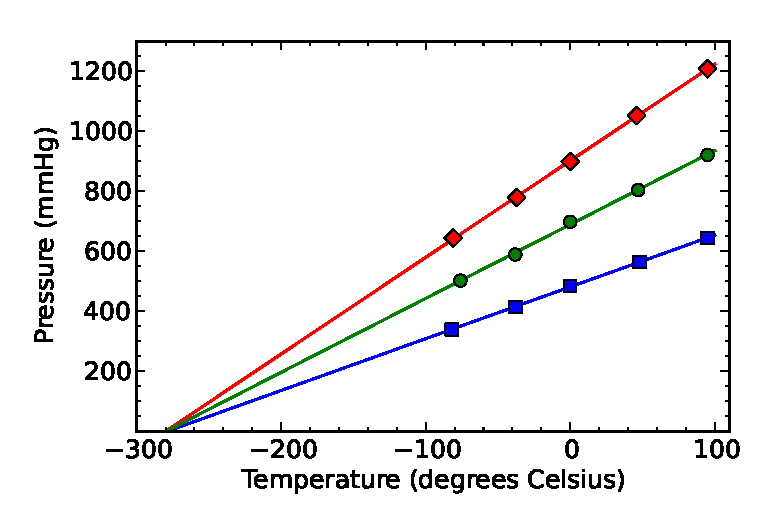
\includegraphics{GasBulbData.eps}
\caption{Pressure as a function of temperature for a fixed volume of air.  
The three data sets are for three different amounts of air in the container. 
For an ideal gas, the pressure would go to zero at $-273^\circ$C.  (Notice
that this is a vector graphic, so it can be viewed at any scale without
seeing pixels.)}
\label{gasbulbdata}
\end{figure}

Most \LaTeX\ implementations can import a variety of graphics formats.
For graphs and line drawings you should use vector (i.e., resolution-independent)
graphics saved in encapsulated PostScript (.eps), scalable vector graphics (.svg), 
or portable document format (.pdf).  Most good graphics software systems can 
save to these formats.  Please don't use a rasterized graphics format
(such as .jpg or .png or .tiff) for graphs or line drawings.

\begin{figure}[h!]
\centering
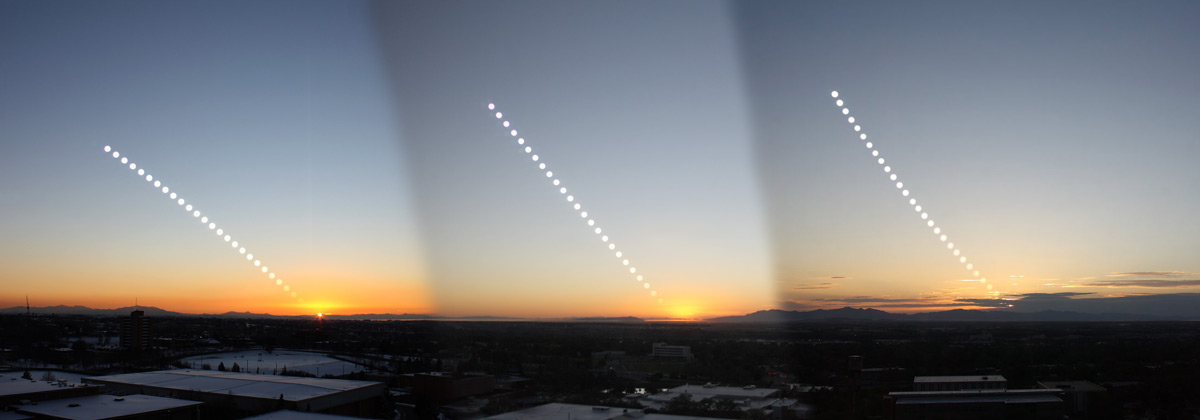
\includegraphics[width=5in]{ThreeSunsets.jpg}
% Notice the width specification.  Photographs should normally have a
% resolution of approximately 300 pixels per inch when printed, that is,
% a total width of about 1000 pixels for a photo to be printed one column
% wide.  Note also that this included photo is in .jpg format even though 
% a .tiff version should be submitted for final production.
\caption{Three overlaid sequences of photos of the setting sun, taken
near the December solstice (left), September equinox (center), and
June solstice (right), all from the same location at 41$^\circ$ north
latitude. The time interval between images in each sequence is approximately
four minutes.}
\label{sunsets}
\end{figure}

For photographs and other images that are \textit{inherently} made 
of pixels (that is, rasters or bitmaps), \LaTeX\ can 
(usually) handle the .jpg and .png formats as well as .eps and .pdf.  
Figure~\ref{sunsets} is a .jpg example. For final production, however, 
AJP prefers that raster images be in .tiff format.  Most \LaTeX\ systems 
can't import .tiff images, so we recommend using .png or .jpg with \LaTeX\ 
for your initial submission, while saving a higher-quality .tiff version 
to submit as a separate file after your manuscript is conditionally accepted
for publication.

Please refer to the AJP editor's web site\cite{editorsite} for more details 
on AJP's requirements for figure preparation.


\section{Tables}

Tables are somewhat similar to figures:  You use the \texttt{table} environment
to let them ``float'' to an appropriate location, and to automatically number
them and format their captions.  But whereas the content of a figure comes
from an external file, the content of a table is typeset directly in \LaTeX.
For that you use the \texttt{tabular} environment, which uses \verb/&/ and
\verb/\\/ for tabbing and ending rows, just like the \texttt{matrix} and
\texttt{eqnarray} environments discussed in Section~\ref{DispEqSection}.

Table~\ref{bosons} shows a fairly simple example.  Notice that the caption comes
before the table itself, so it will appear above the table instead of below.
The \texttt{ruledtabular} environment, which surrounds \texttt{tabular},
provides the double horizontal lines at the top and bottom, and stretches
the table horizontally out to the margins.  (This will look funny for tables
intended to fill only one column of a final journal page, but there's no 
need to worry about such cosmetic details.)

\begin{table}[h!]
\centering
\caption{Elementary bosons}
\begin{ruledtabular}
\begin{tabular}{l c c c c p{5cm}}
% The codes above determine the horizontal alignment in each column.
% Options are l (left), r (right), c (centered), and p (paragraph).
% The p option allows an entry to be broken into multiple lines, and
% therefore requires a width specification, in this case 5 centimeters.
Name & Symbol & Mass (GeV/$c^2$) & Spin & Discovered & Interacts with \\
\hline	% horizontal line to separate headings from data
Photon & $\gamma$ & \ \ 0 & 1 & 1905 & Electrically charged particles \\
Gluons & $g$ & \ \ 0 & 1 & 1978 & Strongly interacting particles (quarks and gluons) \\
Weak charged bosons & $W^\pm$ & \ 82 & 1 & 1983 & Quarks, leptons, $W^\pm$, $Z^0$, $\gamma$ \\
Weak neutral boson & $Z^0$ & \ 91 & 1 & 1983 & Quarks, leptons, $W^\pm$, $Z^0$ \\
Higgs boson & $H$ & 126 & 0 & 2012 & Massive particles (according to theory) \\
\end{tabular}
\end{ruledtabular}
\label{bosons}
\end{table}
% Tables, like figure captions, should be moved to the end when you submit 
% an editable manuscript for production, after conditional acceptance.
% Put the tables after the endnotes but before the figure captions.

Every table is a little bit different, and many tables will require
further tricks; see Refs.\ \onlinecite{wikibook} and~\onlinecite{latexbook}
for examples.  Note that the AJP style does not ordinarily use lines 
to separate rows and columns in the body of a table.


\section{Special formats}

\subsection{Block quotes}  % In subsection headings, only the first word is capitalized.

If a quoted passage is long or important, you can use the \texttt{quote} 
environment to typeset it as a block quote, as in this passage from The 
Feynman Lectures:\cite{feynman}
\begin{quote}
A poet once said, ``The whole universe is in a glass of wine.'' We will 
probably never know in what sense he meant that, for poets do not write 
to be understood. But it is true that if we look at a glass of wine closely 
enough we see the entire universe.
\end{quote}

\subsection{Numbered lists}

To create a numbered list, use the \texttt{enumerate} environment and start
each entry with the \verb/\item/ macro:
\begin{enumerate}
\item You can't win.
\item You can't even break even.
\item You can't get out of the game.
\end{enumerate}

\subsection{Unnumbered lists}

For a bulleted list, just use \texttt{itemize} instead of \texttt{enumerate}:
\begin{itemize}
\item Across a resistor, $\Delta V = \pm IR$.
\item Across a capacitor, $\Delta V = \pm Q/C$.
\item Across an inductor, $\Delta V = \pm L(dI/dt)$.
\end{itemize}

\subsection{Literal text}

For typesetting computer code, the \texttt{verbatim} environment reproduces
every character verbatim, in a typewriter font:
\begin{verbatim}
    u[t_] := NIntegrate[
        x^2 * Sqrt[x^2+t^-2] / (Exp[Sqrt[x^2+t^-2]] + 1), {x,0,Infinity}]
    f[t_] := NIntegrate[
        x^2 * Log[1+ Exp[-Sqrt[x2+t^-2]]], {x,0,Infinity}]
    Plot[((11Pi^4/90) / (u[t]+f[t]+(2Pi^4/45)))^(1/3), {t,0,3}]
\end{verbatim}
There's also a \verb/\verb/ macro for typesetting short snippets of verbatim
text within a paragraph. To use this macro, pick any character that doesn't
appear within the verbatim text to use as a delimiter. Most of the examples
in this article use \texttt{/} as a delimiter, but in \verb|{a/b}| we've used
\verb/|/ instead.


\section{Endnotes and references}

This article has already cited quite a few endnotes, using the \verb/\cite/
macro. See the end of this article (and source file) for the endnotes
themselves, which are in an environment called \texttt{thebibliography}
and are created with the \verb/\bibitem/ macro.  These macros require
you to give each endnote a name.  The notes will be numbered in the
order in which the \verb/\bibitem/ entries appear, and AJP requires that
this order coincide with the order in which the notes are first cited in 
the article.  You can cite multiple endnotes in a single \verb/\cite/, 
separating their names by commas.  And you can cite each note as many 
times as you like.

Notice that in the AJP (and Physical Review B) style, the citation numbers 
appear as superscripts. Think carefully about the optimal placement of
each citation, and try not to attach citations to math symbols where the
numbers might be misinterpreted as exponents. Often there will be a
punctuation symbol after the word where you attach the citation; you
should then put the citation \textit{after} the punctuation, not 
before.\cite{nevermindlogic}

If you want to refer directly to Ref.~\onlinecite{mermin} (or any other) 
in a sentence, you can do so with the \verb/\onlinecite/ macro.

Most endnotes consist of bibliographic citations.\cite{noBIBTeX}  Be sure 
to learn and use the AJP styles for citing books,\cite{latexbook} 
articles,\cite{dyson} edited volumes,\cite{examplevolume} and
URLs.\cite{latexsite}  For example, article titles are in double quotes, 
while book titles are in italics. Pay careful attention to all punctuation 
symbols in citations.  Note that AJP requires that all article citations 
include titles as well as beginning and ending page numbers.
Please use standard abbreviations, as listed in the AIP Style 
Manual,\cite{AIPstylemanual} for journal titles.


\section{Conclusion}

We hope this article will help you prepare beautifully typeset
manuscripts for the American Journal of Physics.  Good typesetting requires
considerable attention to detail, but this effort will pay off by making your
manuscript easier and more enjoyable to read.  Your colleagues, reviewers, 
and editors will be grateful for your effort.

Of course, we encourage you to put as much care into the \textit{content} 
of your manuscript as you put into its form.  The AIP Style 
Manual\cite{AIPstylemanual} is an indispensable reference on good physics 
writing, covering everything from planning and organization to standard 
spellings and abbreviations.

Most important of all, please familiarize yourself with the AJP Statement
of Editorial Policy,\cite{editorsite} which describes the types of manuscripts 
that AJP publishes and the audience for which AJP authors are expected to write.
You wouldn't want to put all that care into preparing a manuscript for AJP,
only to find that AJP is the wrong journal for your manuscript.

We look forward to receiving your submission to AJP.


\appendix*   % Omit the * if there's more than one appendix.

\section{Uninteresting stuff}

Appendices are for material that is needed for completeness but
not sufficiently interesting to include in the main body of the paper.  Most
articles don't need any appendices, but feel free to use them when
appropriate.  This sample article needs an appendix only to illustrate how 
to create an appendix.


\begin{acknowledgments}

We gratefully acknowledge Harvey Gould and Jan Tobochnik, who created an earlier 
AJP \LaTeX\ sample article that inspired this one.  This work was supported by the 
American Association of Physics Teachers.

\end{acknowledgments}


\begin{thebibliography}{99}
% The numeral (here 99) in curly braces is nominally the number of entries in
% the bibliography. It's supposed to affect the amount of space around the
% numerical labels, so only the number of digits should matter--and even that
% seems to make no discernible difference.

\bibitem{latexsite} \LaTeX\ Project Web Site, \url{<http://www.latex-project.org/>}.

\bibitem{wikibook} \textit{\LaTeX} (Wikibook), \url{<http://en.wikibooks.org/wiki/LaTeX/>}.

\bibitem{latexbook}Helmut Kopka and Patrick W. Daly, \textit{A Guide to
\LaTeX}, 4th edition (Addison-Wesley, Boston, 2004).

\bibitem{revtex} REV\TeX\ 4 Home Page, \url{<https://authors.aps.org/revtex4/>}.

\bibitem{cloudLaTeX} On the other hand, you can avoid the installation process
entirely by using a cloud-based \LaTeX\ processor such as Overleaf,
\url{<https://www.overleaf.com/>}.

\bibitem{nevermindlogic} In typography, aesthetics often takes precedence over logic.

\bibitem{FontEncodingComment} Please don't try to handle foreign characters 
and accents with the \texttt{inputenc} and \texttt{fontenc} packages, which 
are incompatible with AJP's editing process.

\bibitem{wikimathpage} See the Mathematics chapter of Ref.~\onlinecite{wikibook}
for an excellent overview of math symbols and equations, with examples.

\bibitem{labelnames} Thinking up a good label name takes a moment, but 
it's worth the trouble; we strongly advise against using labels like 
\texttt{eq2}, which become extremely confusing after you decide to add 
another equation before Eq.~(\ref{deriv}).

\bibitem{footnotes} You need to process a file twice to get the counters correct.

\bibitem{mermin} N. David Mermin, ``What's wrong with these equations?,'' 
Phys. Today \textbf{42} (10), 9--11 (1989).  
% Note that the issue number (10) in this citation is required, because
% each issue of Physics Today starts over with page 1.  Also note the use of
% an en-dash (--), not a hyphen (-), for the page range.

\bibitem{editorsite} American Journal of Physics Editor's Web Site, 
\url{<https://ajp.aapt.org/>}.

\bibitem{feynman} Richard P. Feynman, Robert B. Leighton, and Matthew Sands, 
\textit{The Feynman Lectures on Physics, Vol.\ 1} (Addison-Wesley, 1964), p.~3-10.
% Note that this book is paginated by chapter; "3-10" is a single page reference
% that uses a hyphen, not a range of pages that would us an en-dash (--).

\bibitem{noBIBTeX} Many \LaTeX\ users manage their bibliographic data with 
a tool called BIB\TeX.  Unfortunately, AJP cannot accept BIB\TeX\ files; all 
bibliographic references must be incorporated into the manuscript file
as shown here, at least when you send an editable file for production.

\bibitem{dyson} Freeman J. Dyson, ``Feynman's proof of the Maxwell equations,''
Am. J. Phys. \textbf{58} (3), 209--211.  
% The issue number (3) in this citation is optional, because AJP's pagination 
% is by volume.

\bibitem{examplevolume} M. R. Flannery, ``Elastic scattering,'' in 
\textit{Atomic, Molecular, and Optical Physics Handbook}, edited by
G. W. F. Drake (AIP Press, New York, 1996), p.~520.

\bibitem{AIPstylemanual} \textit{AIP Style Manual}, 4th edition (American 
Institute of Physics, New York, 1990). Available online at 
\url{<https://www.aapt.org/Publications/upload/aip_style_4thed.pdf>}. Although parts of 
it have been made out of date by advancing technology, most of this manual 
is still as useful as ever. Just be sure to follow AJP's specific rules
whenever they conflict with those in the manual.

\end{thebibliography}

\end{document}
